% !TeX spellcheck = es_ES
\documentclass[12pt, titlepage]{article}
\usepackage[utf8]{inputenc}
\usepackage[spanish]{babel}
\usepackage{float}
\usepackage[letterpaper, margin=2.5cm]{geometry}
\usepackage[nottoc,notlot,notlof]{tocbibind} % Hace que se agregen las referencias al indice
\usepackage{url}
\usepackage{graphicx} 
\usepackage{listings}
\usepackage{color}
\definecolor{dkgreen}{rgb}{0,0.6,0}
\definecolor{gray}{rgb}{0.5,0.5,0.5}
\definecolor{mauve}{RGB}{253,151,31}

\lstset{frame=tb,
    language=Sql,
    aboveskip=3mm,
    belowskip=3mm,
    showstringspaces=false,
    columns=flexible,
    basicstyle={\small\ttfamily},
    numbers=none,
    numberstyle=\tiny\color{gray},
    keywordstyle=\color{blue},
    commentstyle=\color{dkgreen},
    stringstyle=\color{mauve},
    breaklines=true,
    breakatwhitespace=true,
    tabsize=2,
    morekeywords={use}
}

\title{Reporte: Práctica 5}
\author{Carlos Tonatihu Barrera Pérez \\ Profesor: Hernández Contreras Euler \\ Bases de Datos \\ Grupo: 2CM1 }
\date{31 de marzo de 2017}

\begin{document}
	\maketitle
	\tableofcontents
	\section{Marco Teórico}
	Los sistemas comerciales de bases de datos no usan álgebra relacional, en su lugar utilizan el lenguaje SQL que esta basado en dicha álgebra pero con sintaxis fácil de entender.
	Este lenguaje de definición de datos SQL se utiliza para crear relaciones con esquemas especificados esto es posible ya que el LDD de SQL soporta diferentes tipos de datos y que SQL incluye todas las operaciones del álgebra relacional junto con las operaciones del álgebra relacional extendida.\cite{LIBRO}
	
	Ademas, SQL permite subconsultas anidadas en las cláusulas \textbf{where}. Por su parte las subconsultas de la cláusula \textbf{from} se denominan relaciones derivadas.
	
	Otro punto importante de SQL es que no solo nos permite trabajar consultas, también brinda constructores para actualizar, insertar y borrar información. Finalmente SQL soporta varios tipos de reunión externa con diferentes tipos de condiciones de reunión.\cite{LIBRO}
	
	 \begin{figure}[H]
		\begin{center}
			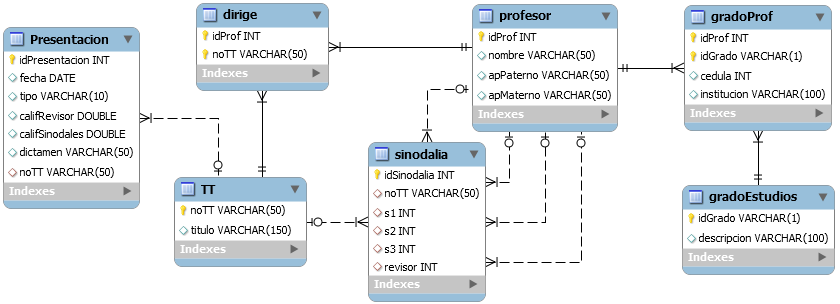
\includegraphics[width=16cm, height=6cm]{img/tt.png}
			\caption{Diagrama de la base de datos usada en esta práctica.}
			\label{fig:home}
		\end{center}
	\end{figure}
\newpage
	\section{Desarrollo}
	Como es costumbre se importo el contenido de la base de datos con la que se iba a trabajar desde un archivo .sql y se procedió a realizar las siguientes consultas.
	
	Primero se mostró el número de TT de aquellos que fueron dirigidos por Andrés Ortigoza.
	
		\begin{figure}[H]
		\begin{center}
			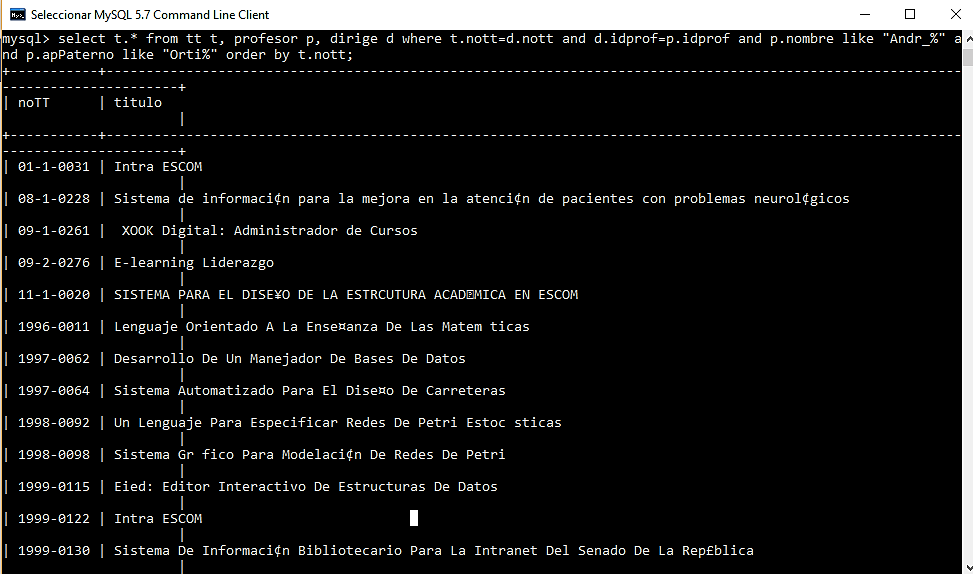
\includegraphics[width=16cm, height=10cm]{img/uno.png}
			\caption{Resultado demasiado grande para mostrarlo en el que se obtuvieron 55 resultados.}
			\label{fig:ejercicio1}
		\end{center}
	\end{figure}
	
	Después se despego toda la información de aquellos TTs que tienen en su titulo "redes neuronales".
	
		\begin{figure}[H]
		\begin{center}
			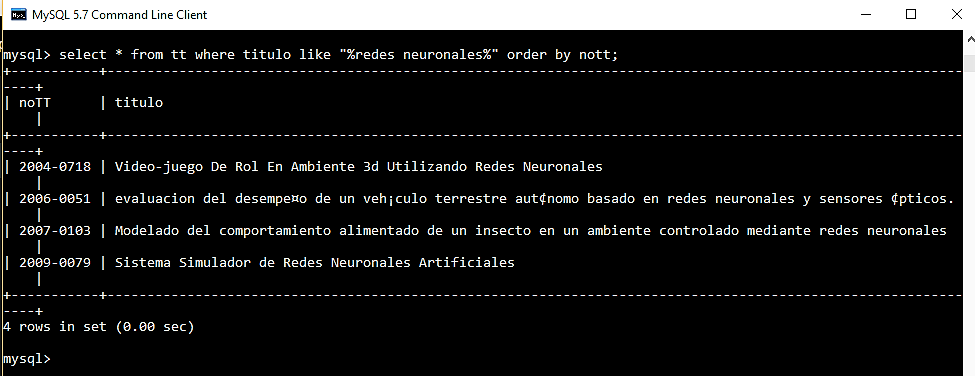
\includegraphics[width=16cm, height=8cm]{img/dos.png}
			\caption{TTs que incluyen redes neuronales en su titulo.}
			\label{fig:dos}
		\end{center}
	\end{figure}
	
	Lo siguiente fue mostrar dictamen y la calificación de los sinodales de aquellos tts que ha dirigido la profesora Fabiola Ocampo.
	
	\begin{figure}[H]
		\begin{center}
			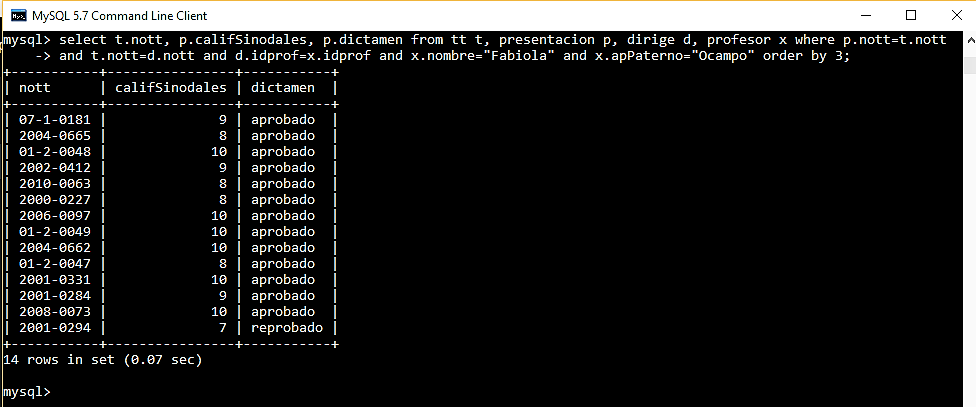
\includegraphics[width=16cm, height=8cm]{img/tres.png}
			\caption{Calificaciones de los tts dirigidos por Fabiola Ocampo.}
			\label{fig:tres}
		\end{center}
	\end{figure}
	
	A continuación se mostró el numero de TT de aquellos profesores que se apellidan Martínez y se incluyo el nombre completo del profesor.
	
	\begin{figure}[H]
		\begin{center}
			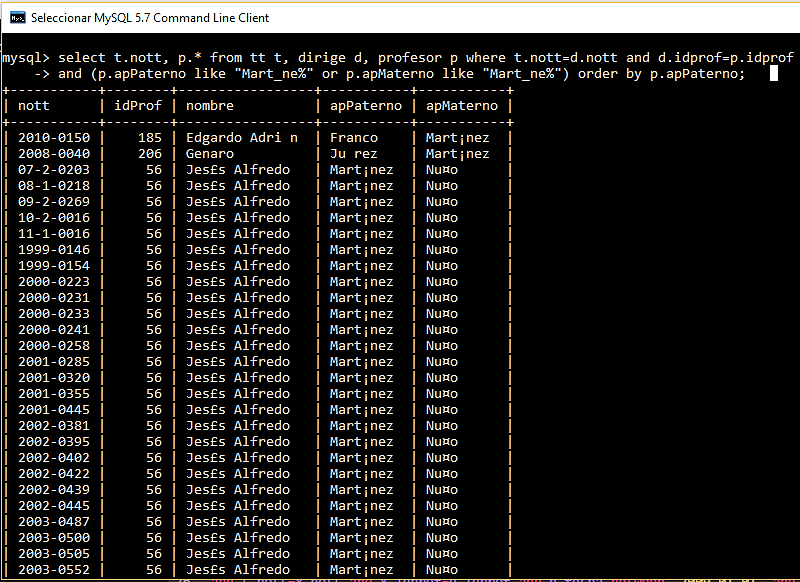
\includegraphics[width=16cm, height=10cm]{img/cuatro.png}
			\caption{La respuesta fue muy grande con 88 resultados.}
			\label{fig:ejercicio5}
		\end{center}
	\end{figure}
	
	Después, se imprimió el grado de estudios que tienen los profesores que se apellidan Maldonado.
	
		\begin{figure}[H]
		\begin{center}
			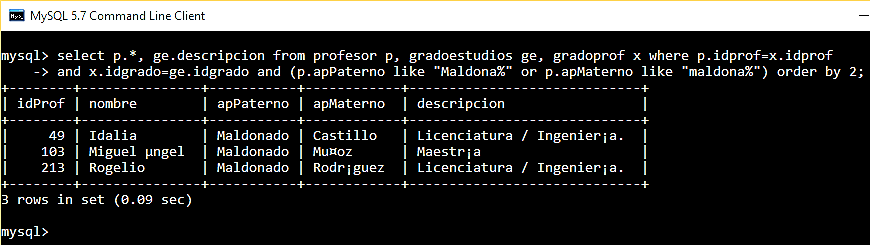
\includegraphics[width=16cm, height=4cm]{img/cinco.png}
			\caption{Profesores con el apellido Maldonado.}
			\label{fig:ejercicio6}
		\end{center}
	\end{figure}
	
	La siguiente acción fue mostrar cuales son los TTs que han reprobado ademas de desplegó sus respectivos directores.
	
	\begin{figure}[H]
		\begin{center}
			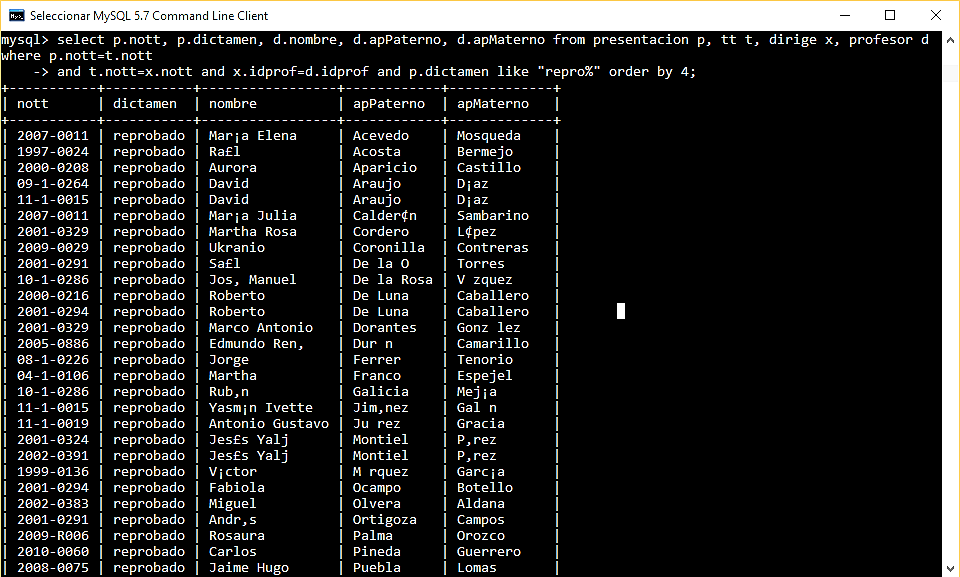
\includegraphics[width=16cm, height=10cm]{img/seis.png}
			\caption{Resultado de la consulta con 36 resultados.}
			\label{fig:ejercicio7}
		\end{center}
	\end{figure}
	
	Luego se desplegó que TTs se han presentado en el año 2009 junto con sus directores.
	
	\begin{figure}[H]
		\begin{center}
			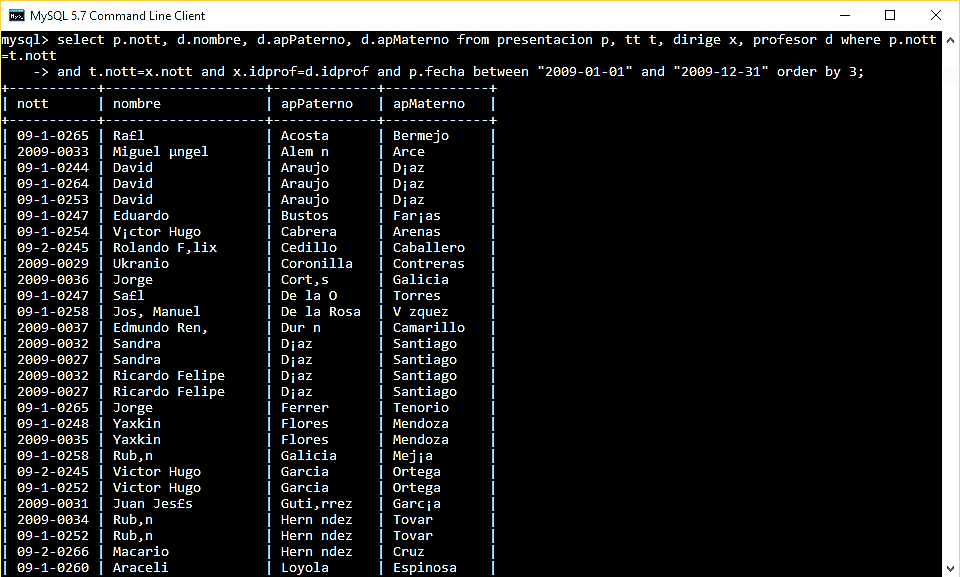
\includegraphics[width=16cm, height=10cm]{img/siete.png}
			\caption{El resultado de esta operación también fue grande con 51 filas.} 
			\label{fig:ejercicio8}
		\end{center}
	\end{figure}
	
	A continuación se imprimió que sinodales tiene el TT 2010-0046.
	\begin{figure}[H]
		\begin{center}
			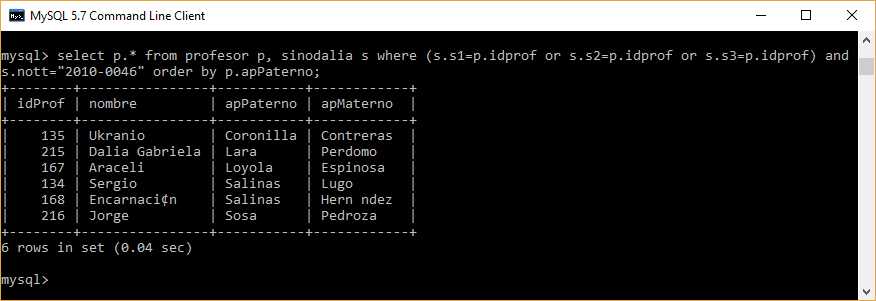
\includegraphics[width=16cm, height=6cm]{img/ocho.png}
			\caption{Sinodales del TT que se indica.} 
			\label{fig:ejercicio9}
		\end{center}
	\end{figure}
	Lo siguiente fue desplegar cuantos TTs ha dirigido el profesor Euler.
	\begin{figure}[H]
		\begin{center}
			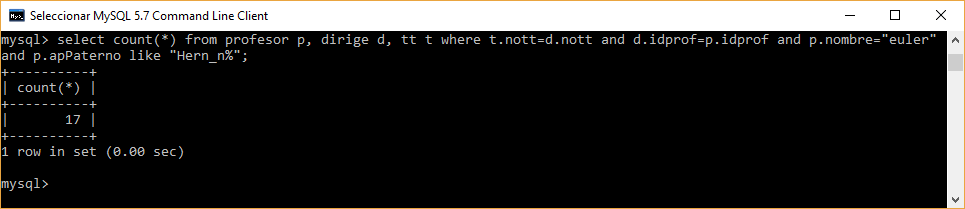
\includegraphics[width=16cm, height=4cm]{img/ultimo2.png}
			\caption{Numero de TTs dirigidos por el profesor Euler.} 
			\label{fig:ejercicio10}
		\end{center}
	\end{figure}
	Ademas, se imprimió el nombre de estos TTs.
	\begin{figure}[H]
		\begin{center}
			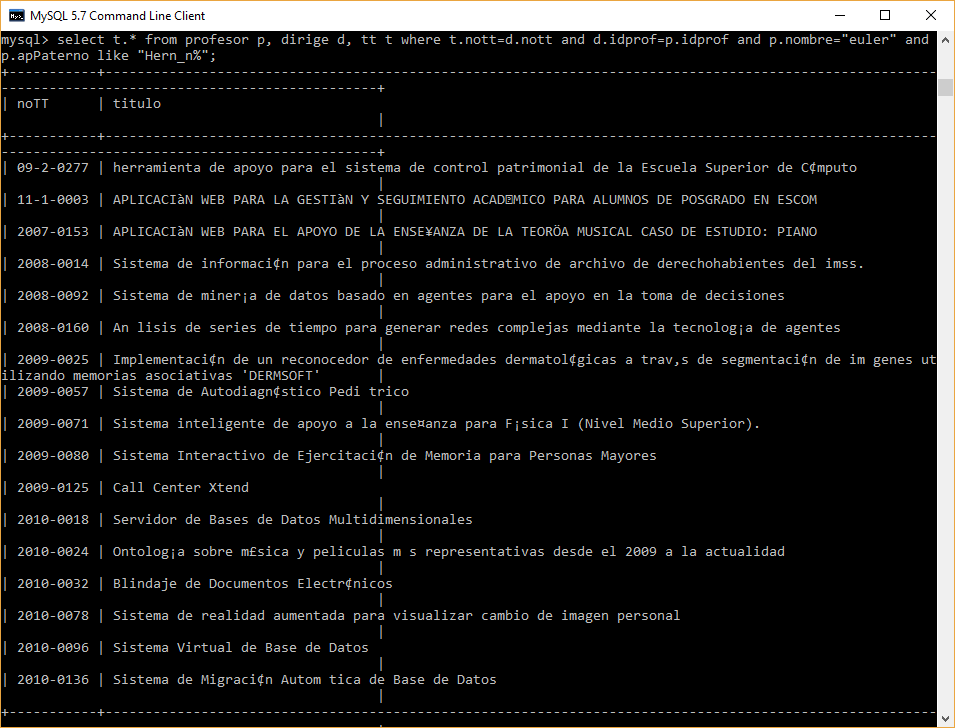
\includegraphics[width=16cm, height=12cm]{img/ultimo1.png}
			\caption{Nombre de los TTs dirigidos por el profesor Euler.} 
			\label{fig:ejercicio11}
		\end{center}
	\end{figure}
	
	Y por ultimo se mostró a los sinodales de dichos TTs.
	\begin{figure}[H]
		\begin{center}
			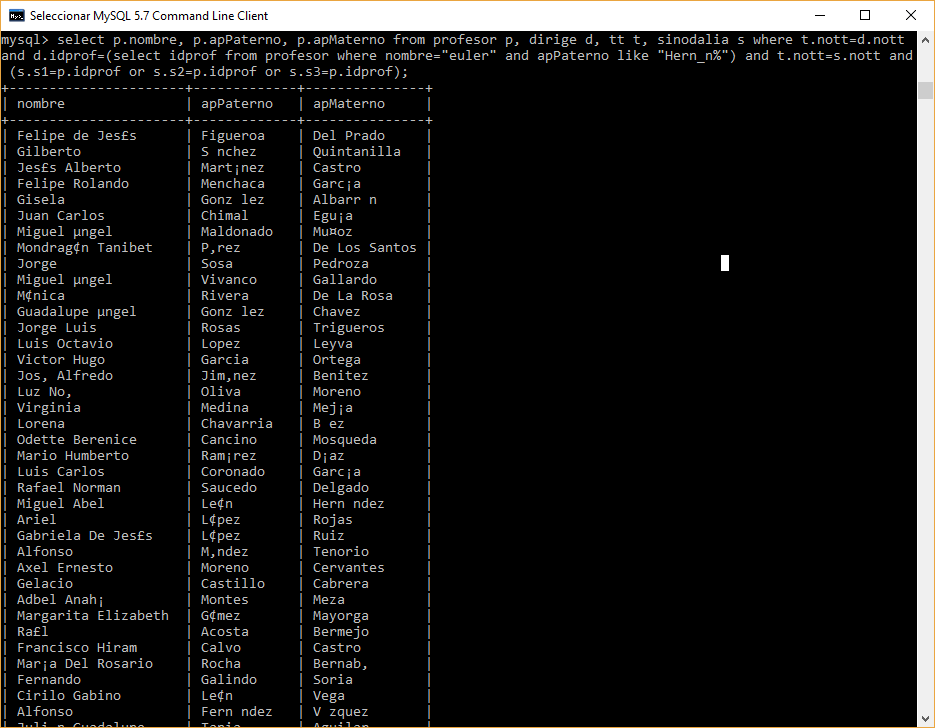
\includegraphics[width=16cm, height=12cm]{img/ultimo.png}
			\caption{En este ultimo ejercicio se obtuvieron 96 resultados.} 
			\label{fig:ultimo}
		\end{center}
	\end{figure}
	\section{Conclusiones}
	Poco a poco las consultas se vuelven más complejas y la ultima realizada en esta práctica es una prueba de ello es por esto que se debe de continuar así para que este tipo de ejercicios no resulten ser un problema y se pueden hacer de la manera más rápida y eficiente posible ya que a la larga el que tan fácil podamos resolver un problema de este tipo determinara la complejidad que podamos alcanzar en los sistemas que se deseen implementar siempre y cuando estos necesiten una base de datos.
	\bibliography{bibliografia} 
	\bibliographystyle{ieeetr}
\end{document}